\section{Appendix}

\begin{figure*}
  \begin{minipage}[t]{0.33\textwidth}
    \centering
    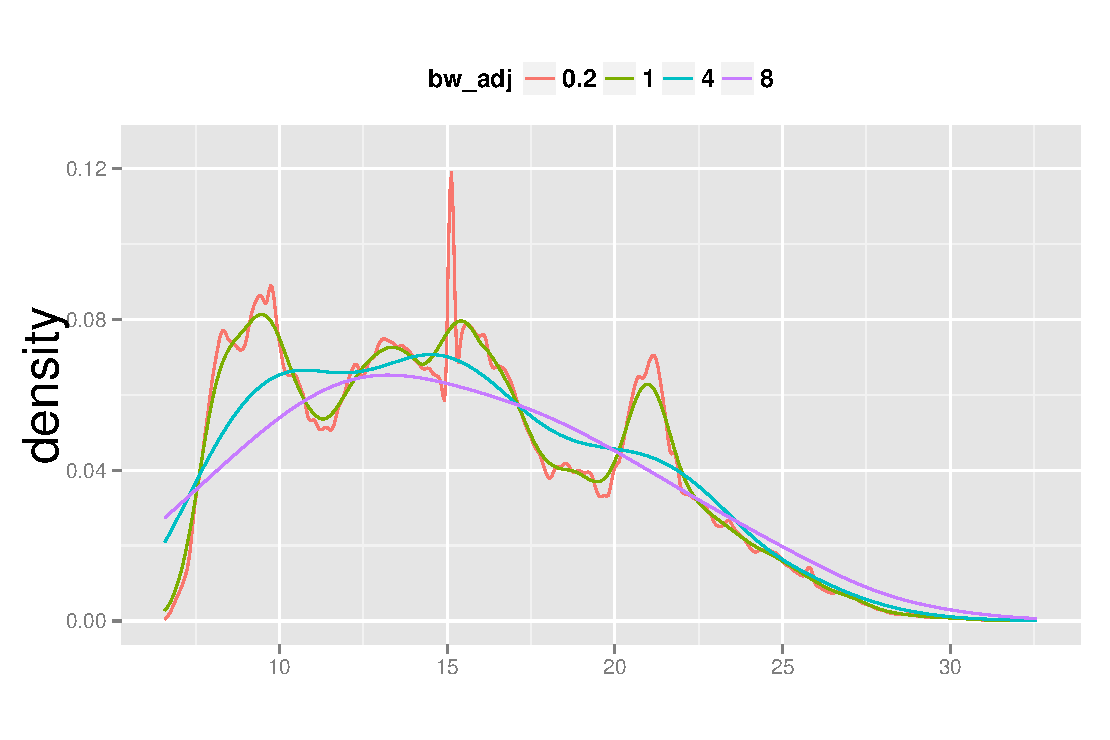
\includegraphics[width=\textwidth,height=\textwidth]{fig/Temperature_biweight.pdf}
    \subcaption{kernel: biweight}
  \end{minipage}
  \begin{minipage}[t]{0.33\textwidth}
    \centering
    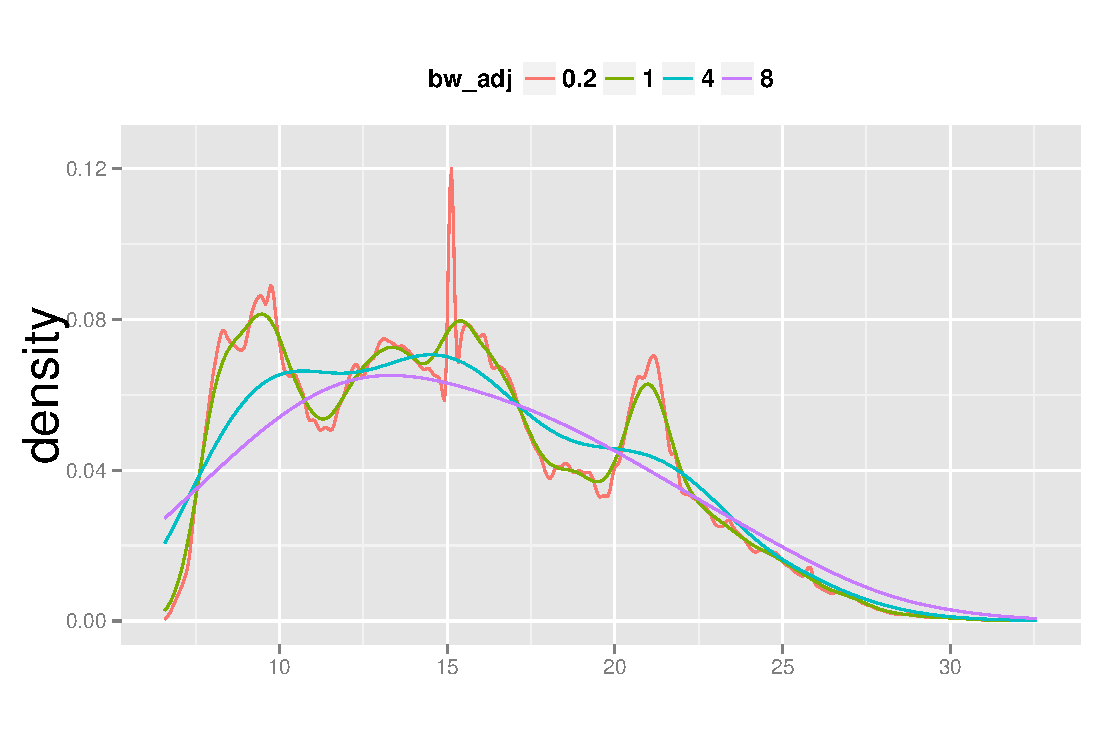
\includegraphics[width=\textwidth,height=\textwidth]{fig/Temperature_cosine.pdf}
    \subcaption{kernel: cosine}
  \end{minipage}
  \begin{minipage}[t]{0.34\textwidth}
    \centering
    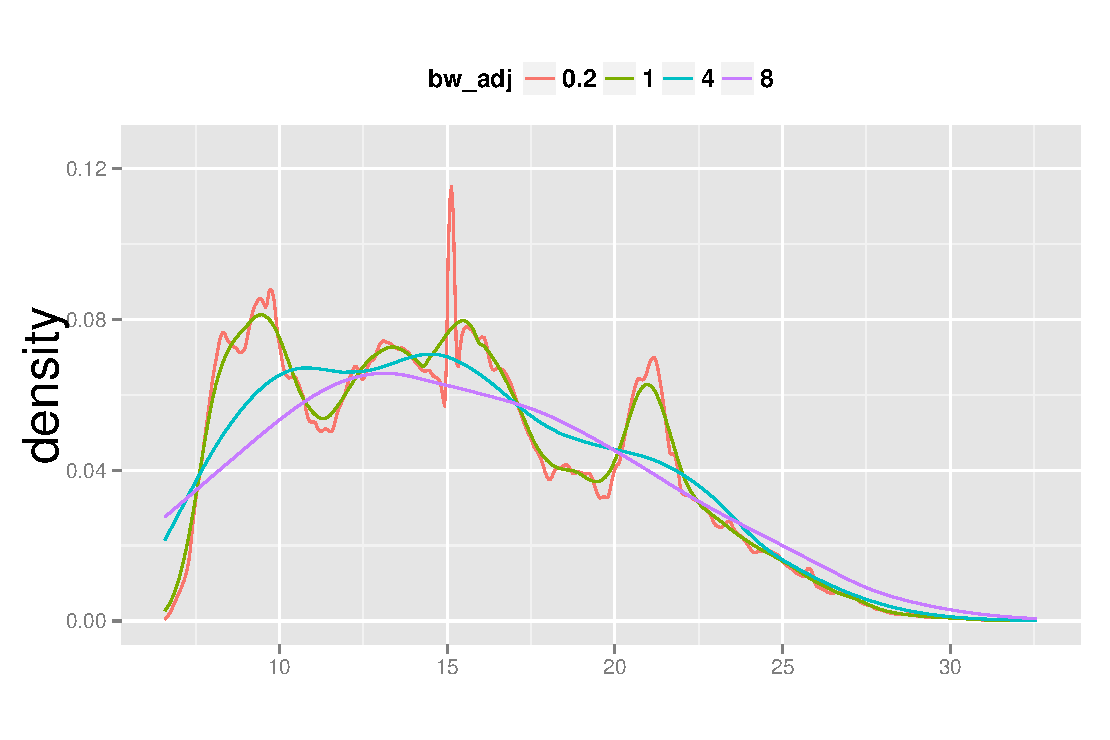
\includegraphics[width=\textwidth,height=\textwidth]{fig/Temperature_epanechnikov.pdf}
    \subcaption{kernel: epanechnikov}
  \end{minipage}\\
    \begin{minipage}[t]{0.33\textwidth}
    \centering
    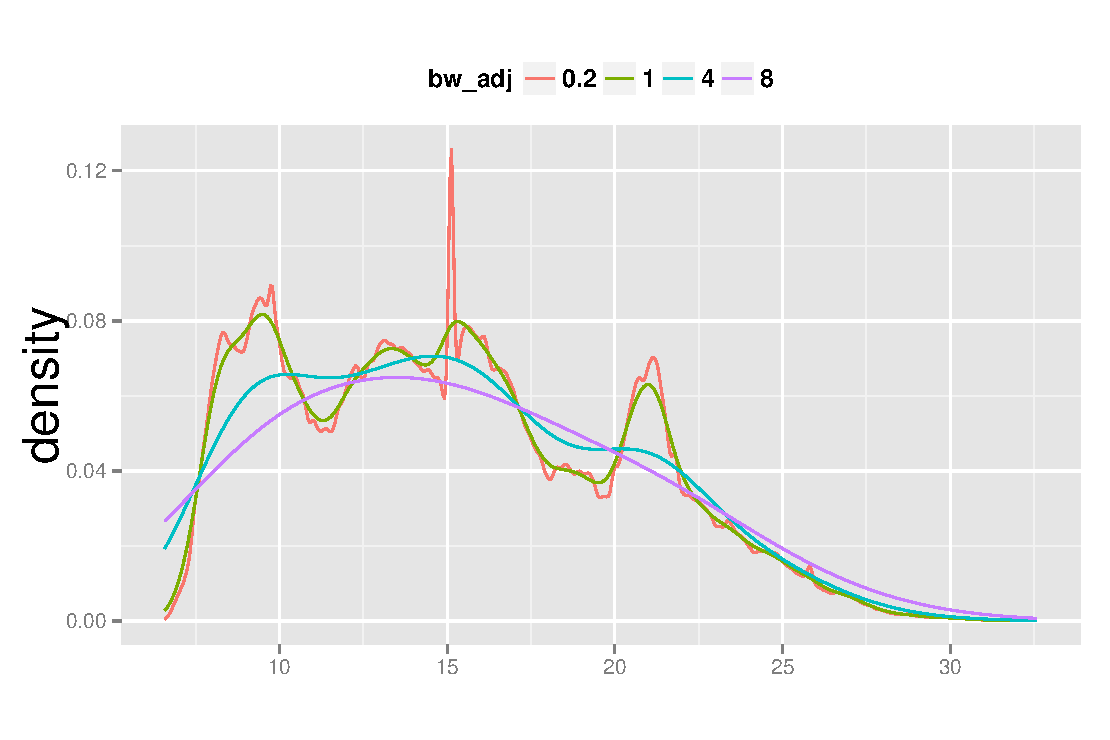
\includegraphics[width=\textwidth,height=\textwidth]{fig/Temperature_Gaussian.pdf}
    \subcaption{kernel: gaussian}
  \end{minipage}
  \begin{minipage}[t]{0.33\textwidth}
    \centering
    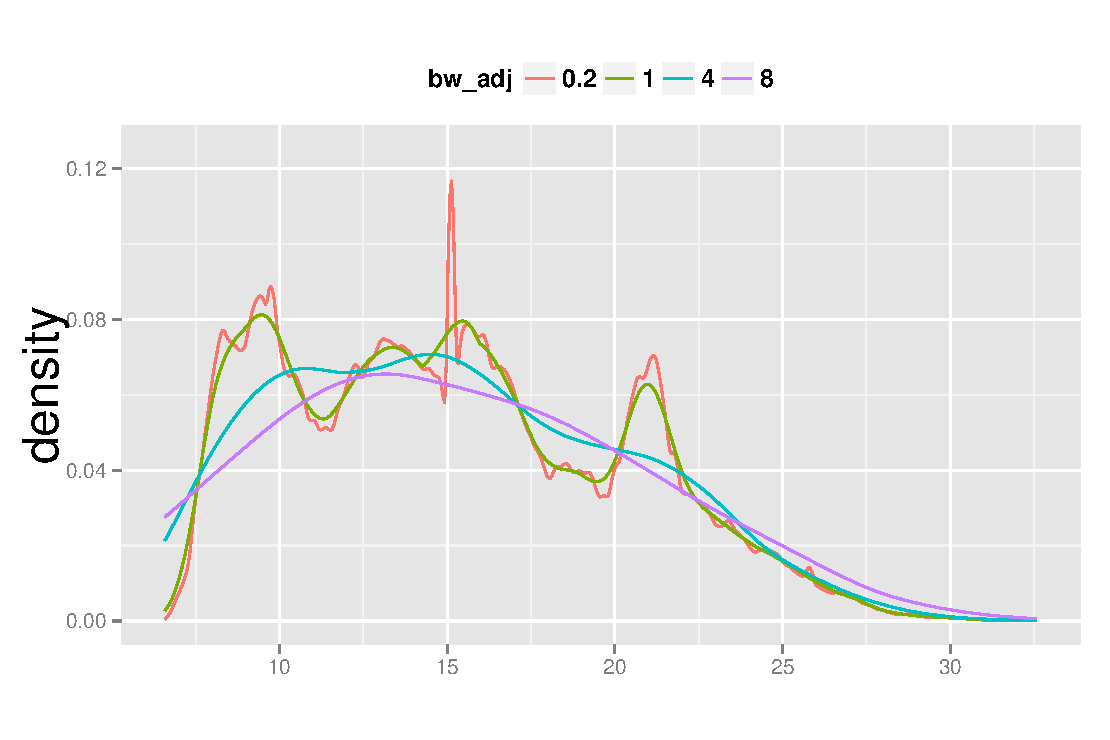
\includegraphics[width=\textwidth,height=\textwidth]{fig/Temperature_optcosine.pdf}
    \subcaption{kernel: optcosine}
  \end{minipage}
  \begin{minipage}[t]{0.34\textwidth}
    \centering
    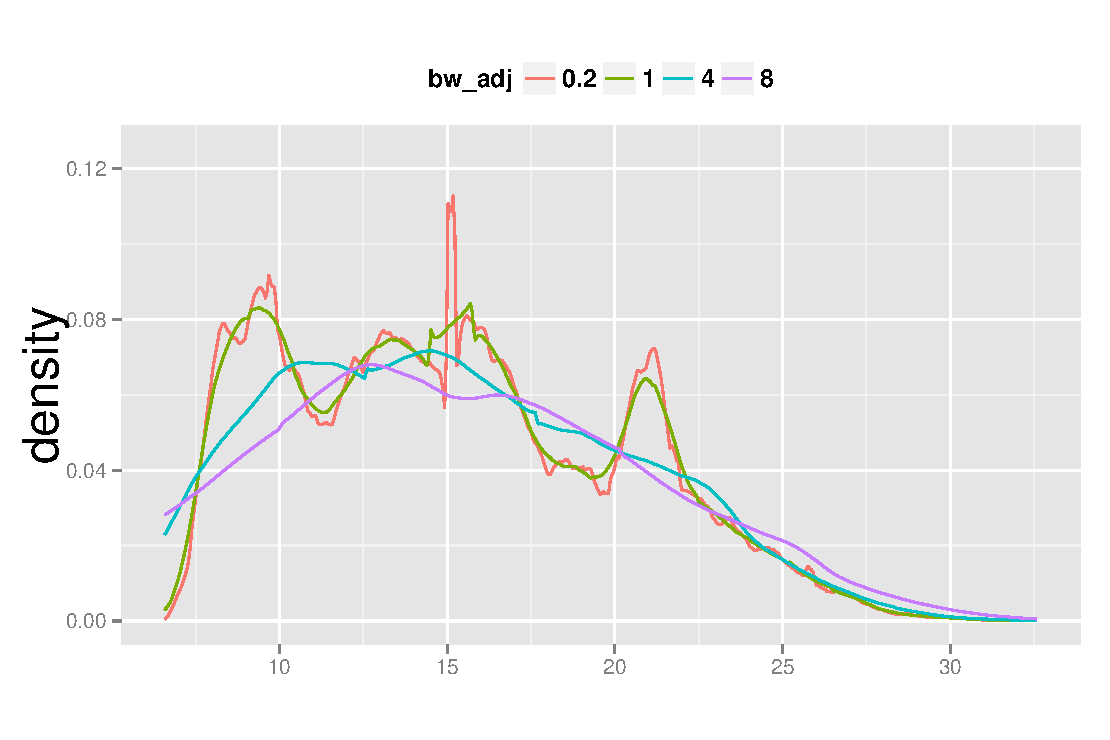
\includegraphics[width=\textwidth,height=\textwidth]{fig/Temperature_rectangular.pdf}
    \subcaption{}
  \end{minipage}\\
  \begin{minipage}[t]{0.33\textwidth}
    \centering
    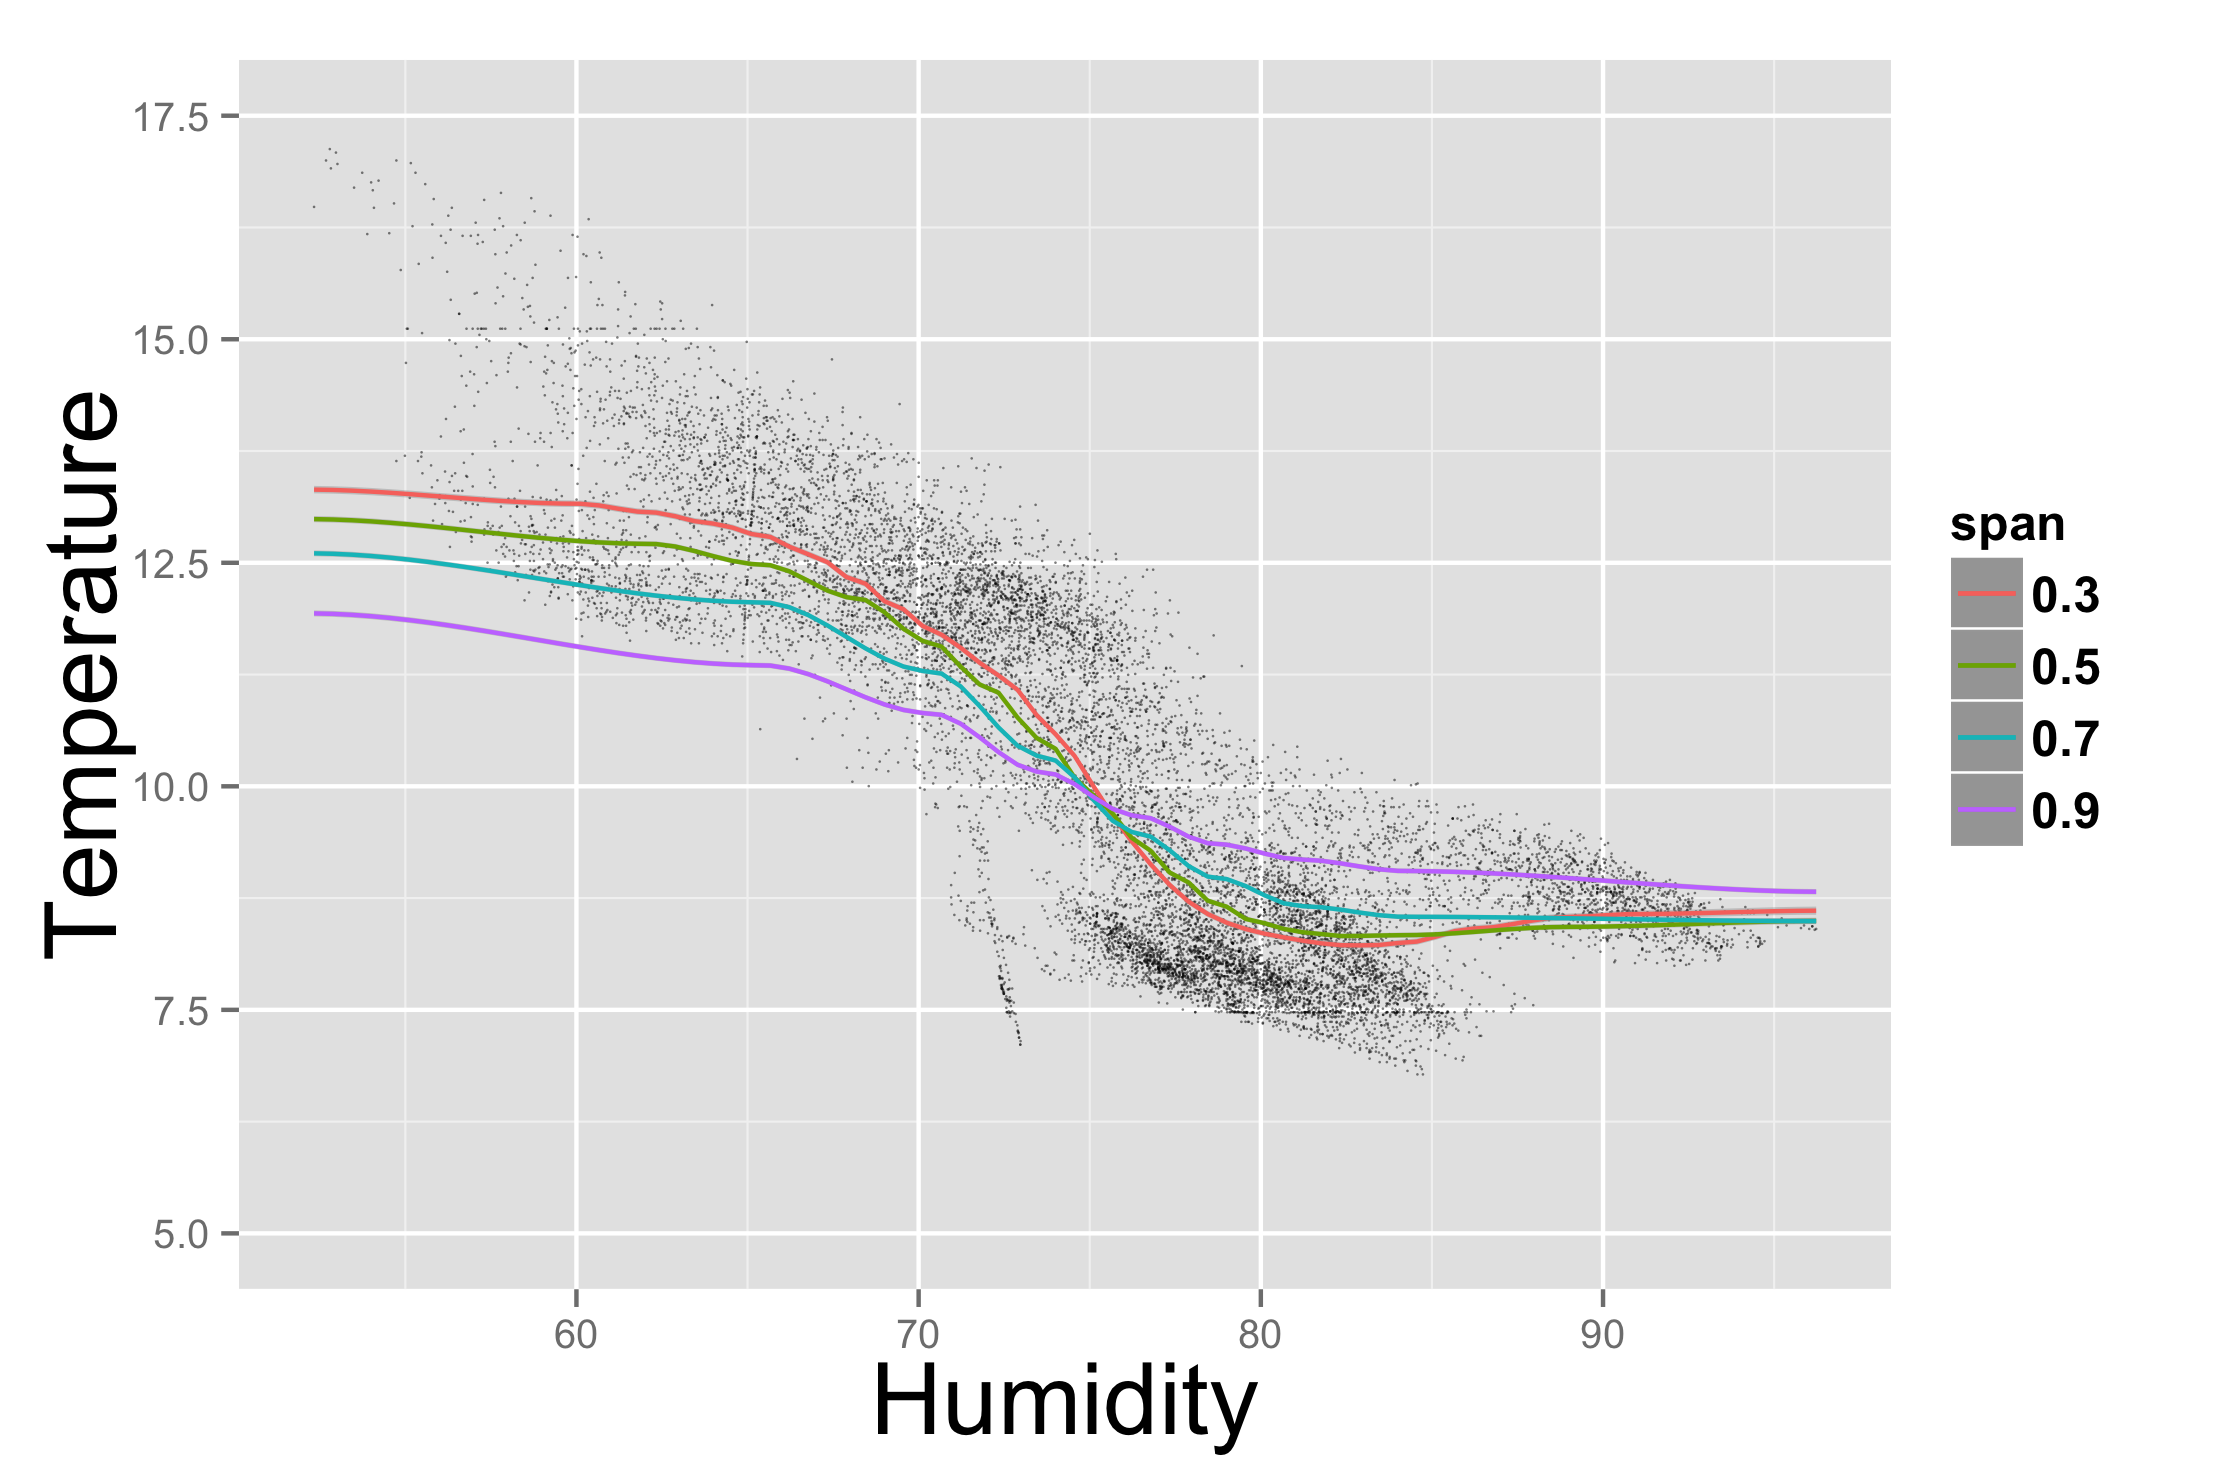
\includegraphics[width=\textwidth,height=\textwidth]{fig/Humid_Temp_Loess_poly0.png}
    \subcaption{degree = 0}
  \end{minipage}
  \begin{minipage}[t]{0.33\textwidth}
    \centering
    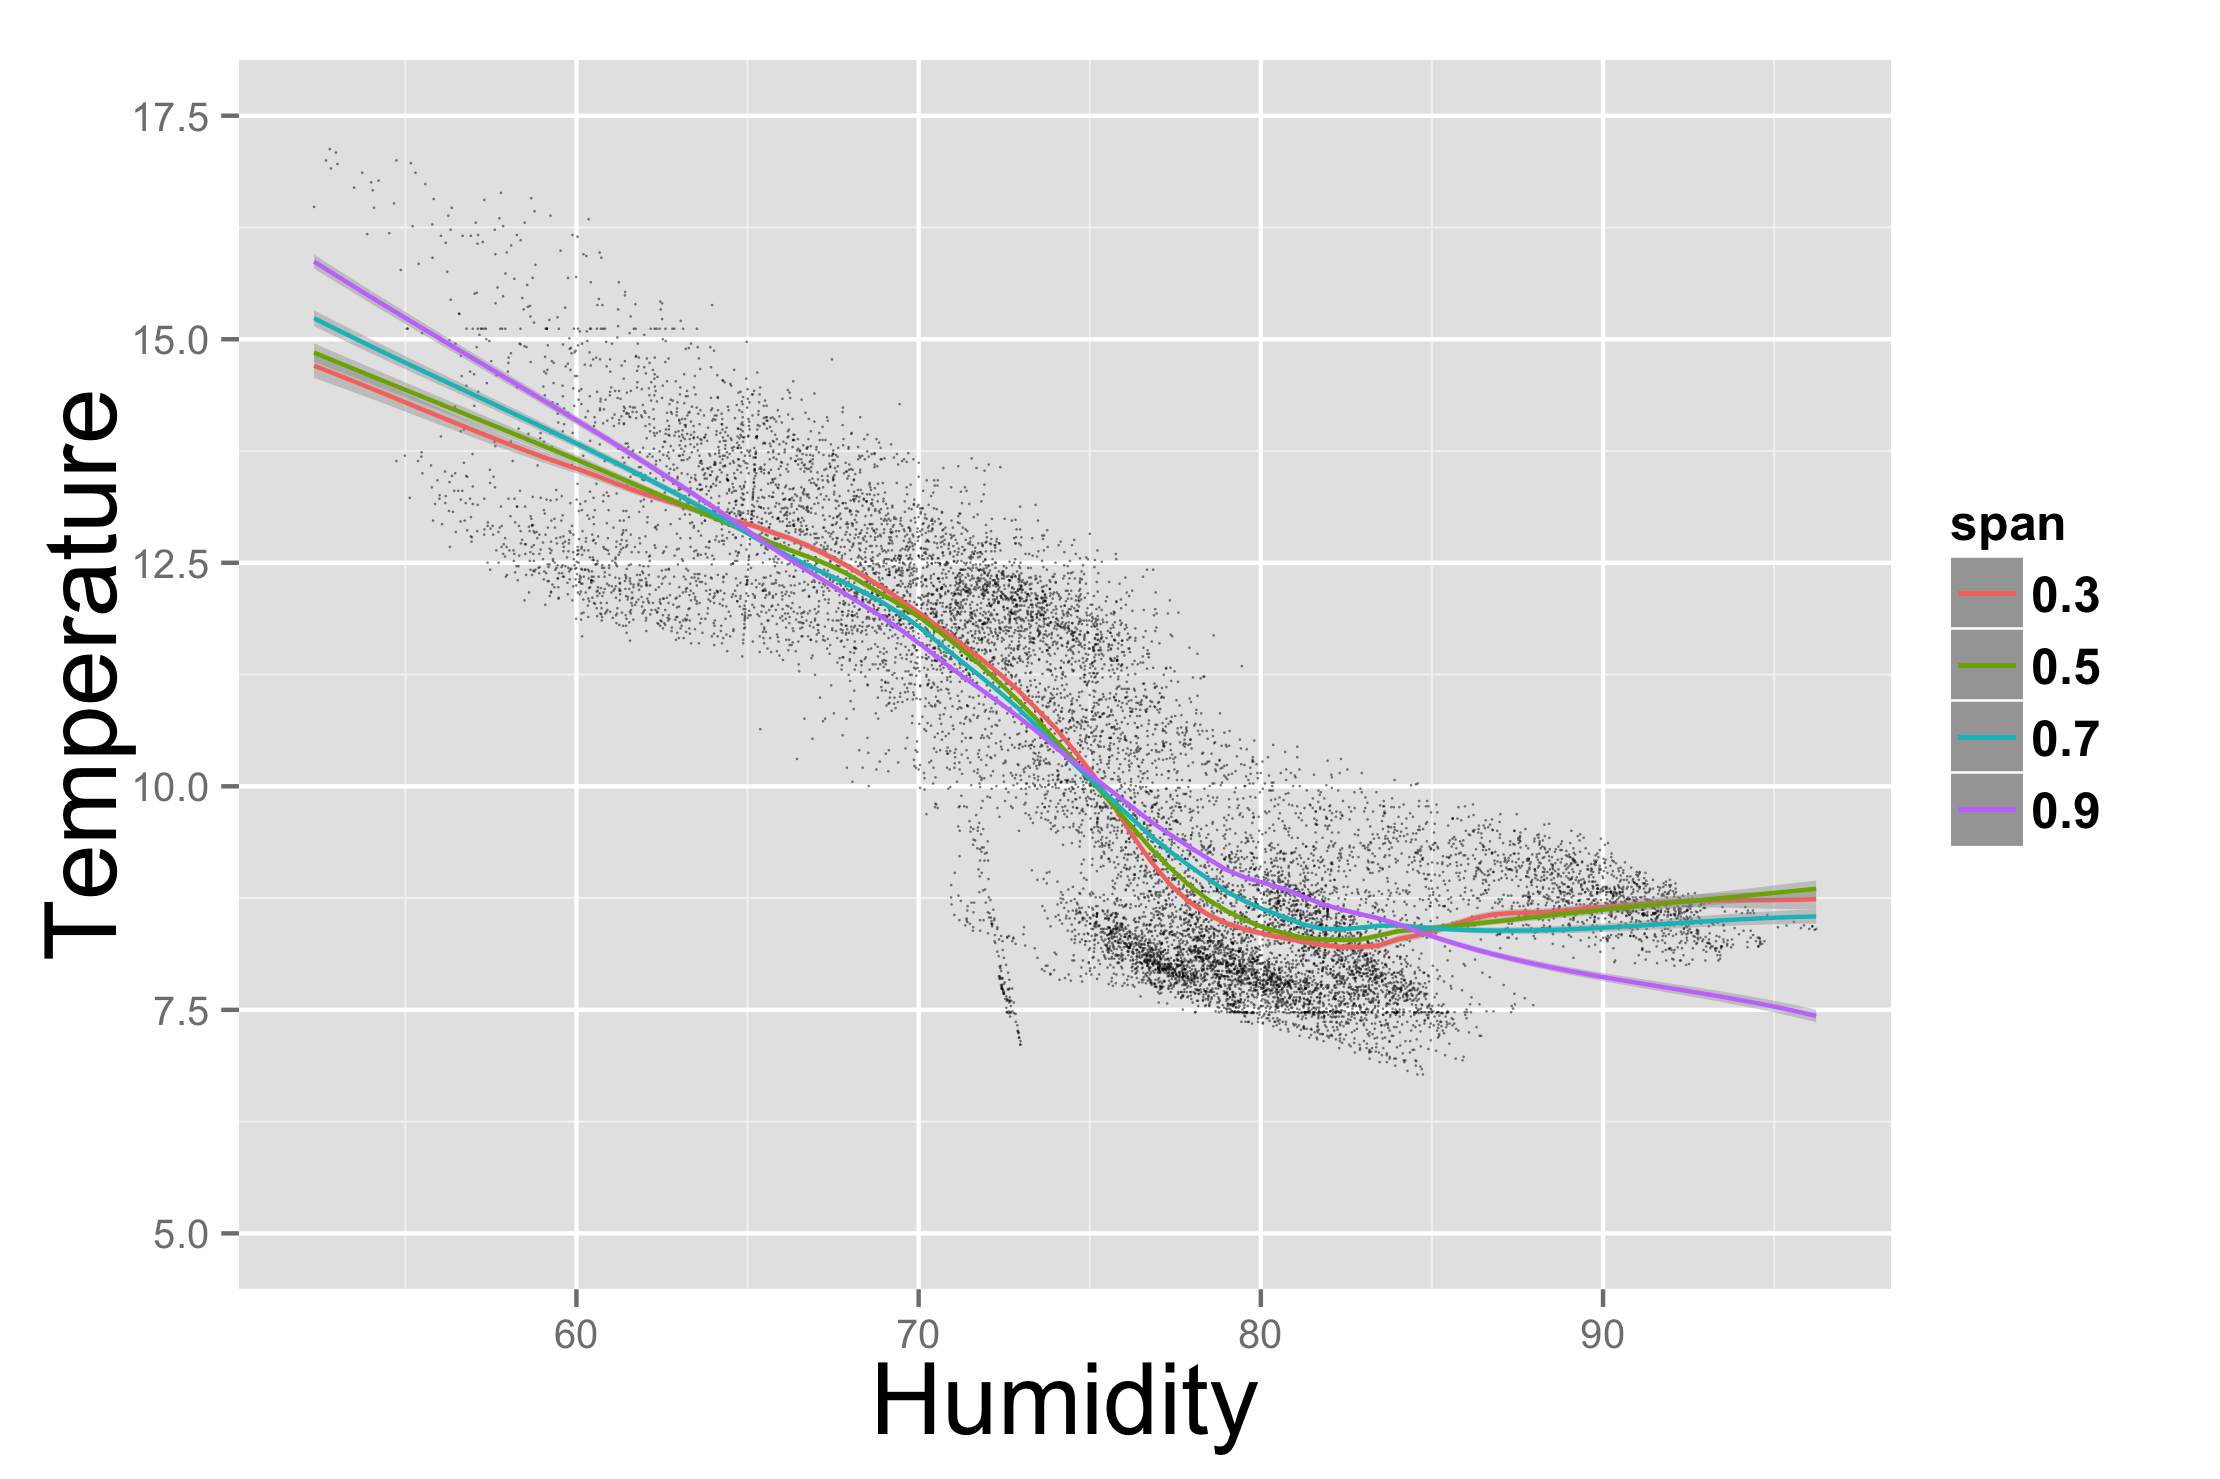
\includegraphics[width=\textwidth,height=\textwidth]{fig/Humid_Temp_Loess_poly1.png}
    \subcaption{degree = 1}
  \end{minipage}
  \begin{minipage}[t]{0.34\textwidth}
    \centering
    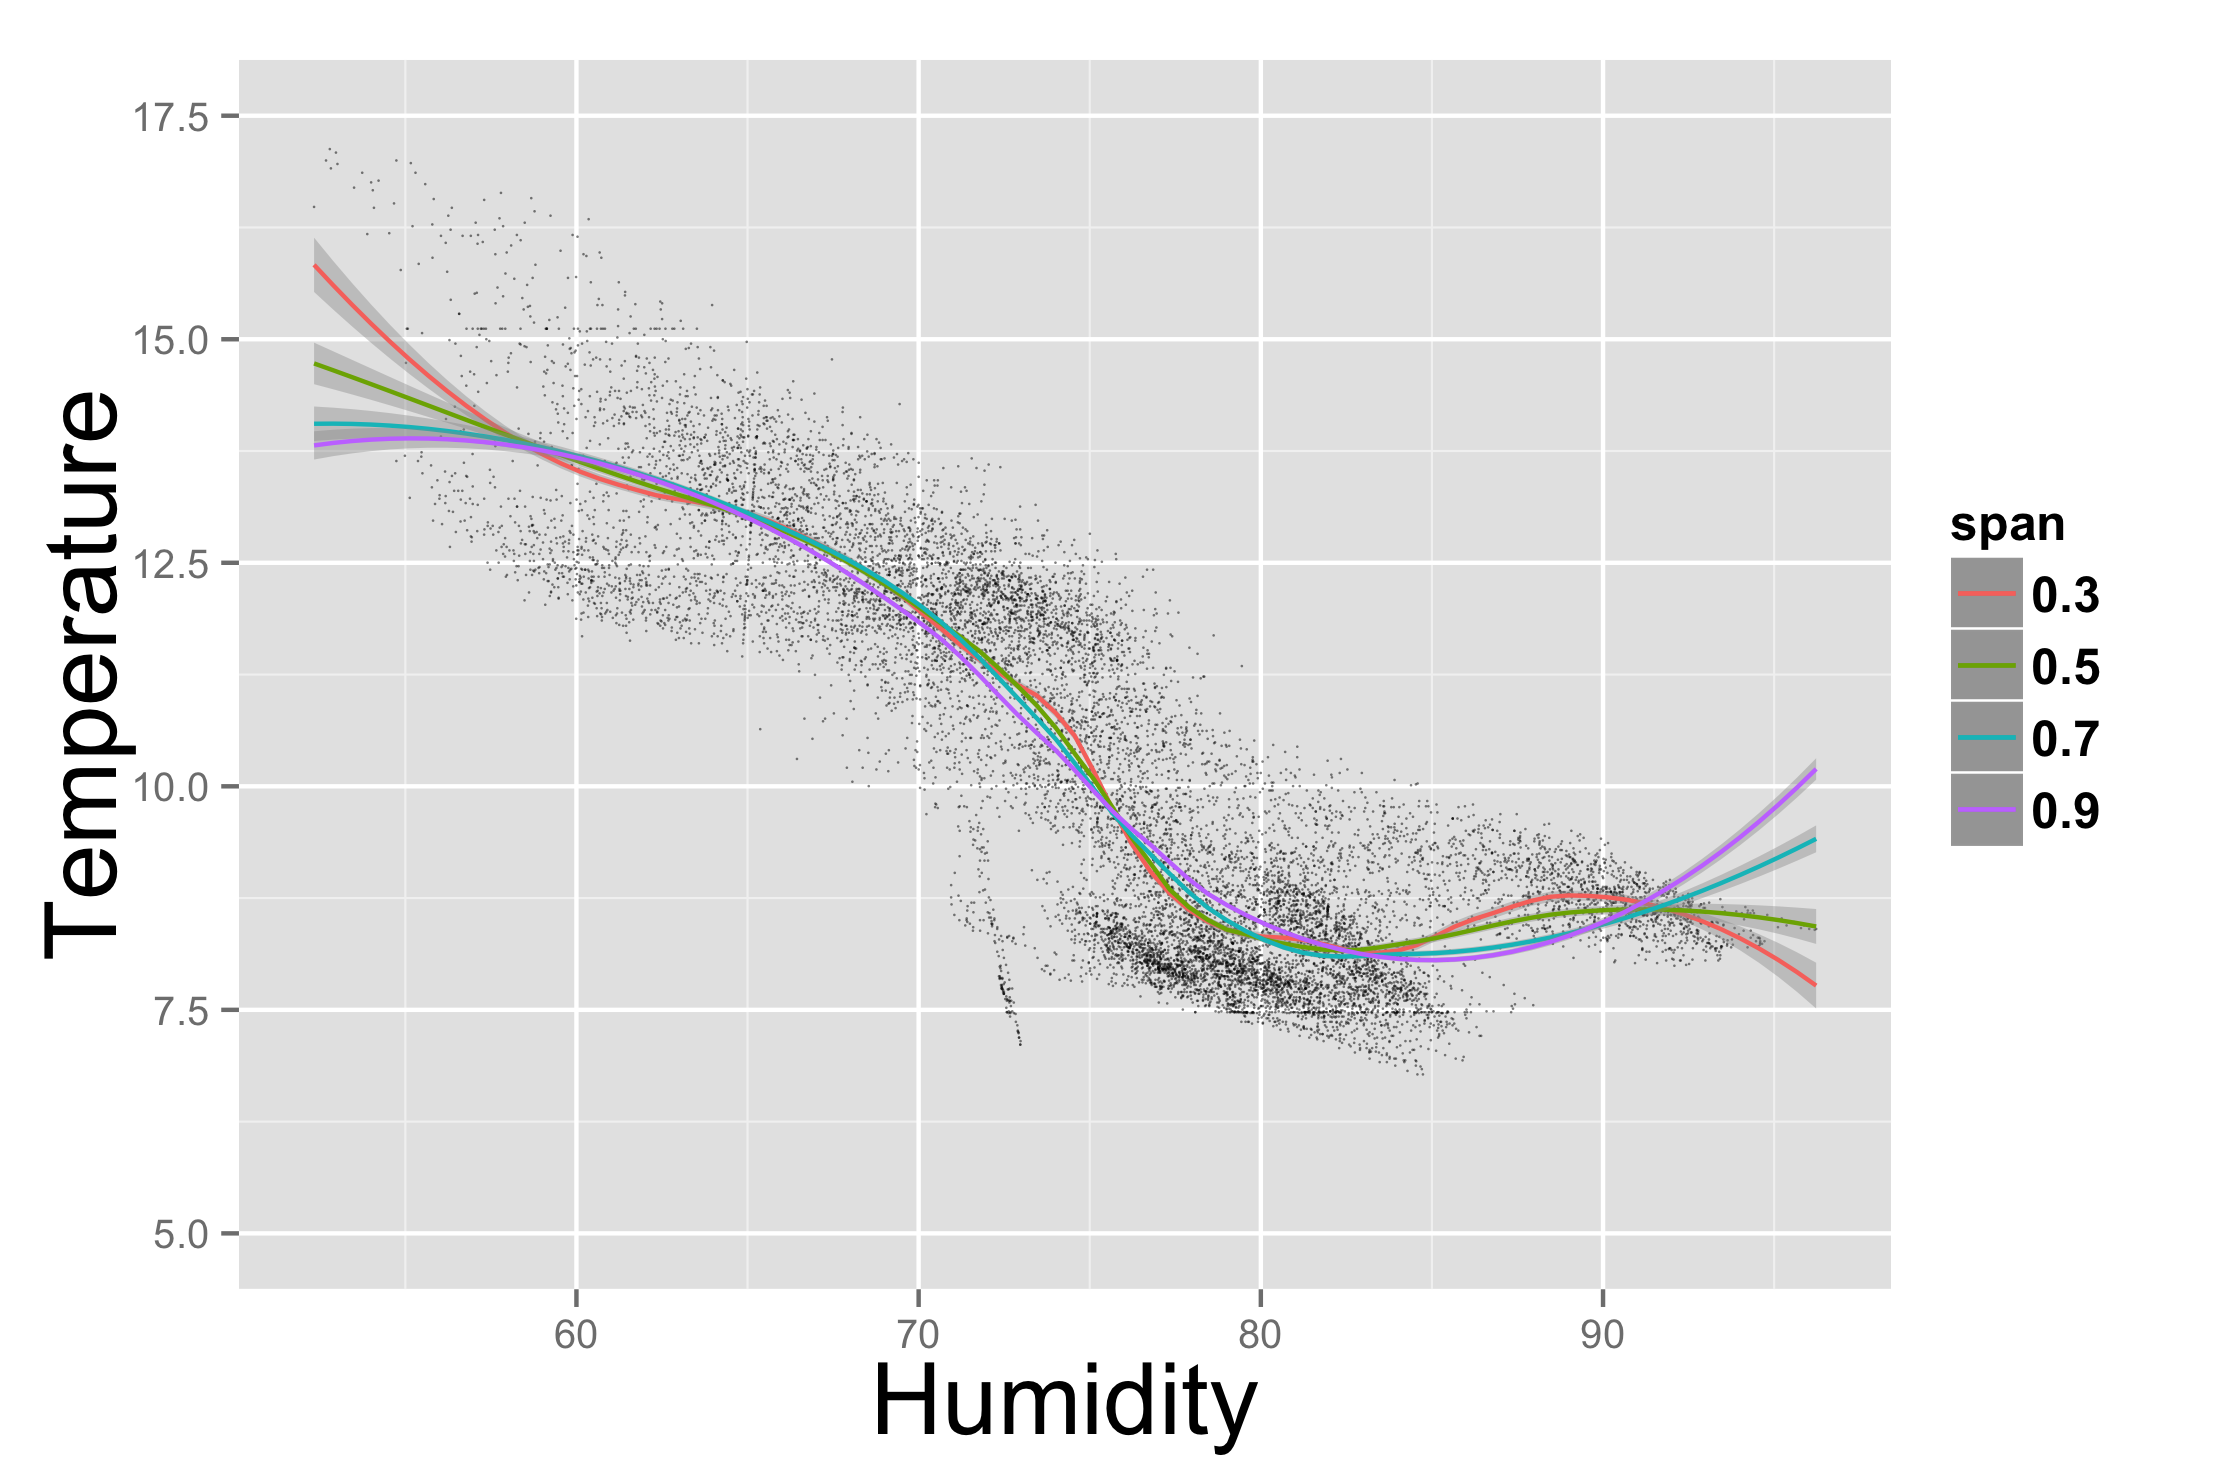
\includegraphics[width=\textwidth,height=\textwidth]{fig/Humid_Temp_Loess_poly2.png}
    \subcaption{degree = 2}
  \end{minipage}\\
  \caption{\textbf{Kernel density and LOESS.}(a)-(f) Kernel density for temperature measurements. (g)-(k) LOESS on the relationship between Temperature and Humidity.}   
  \label{fig:Kernel_LOESS}
\end{figure*}
